\documentclass[12pt, titlepage]{article}

\usepackage{amsmath, mathtools}

\usepackage[round]{natbib}
\usepackage{amsfonts}
\usepackage{amssymb}
\usepackage{graphicx}
\usepackage{colortbl}
\usepackage{xr}
\usepackage{hyperref}
\usepackage{longtable}
\usepackage{xfrac}
\usepackage{tabularx}
\usepackage{float}
\usepackage{siunitx}
\usepackage{booktabs}
\usepackage{multirow}
\usepackage[section]{placeins}
\usepackage{caption}
\usepackage{fullpage}
\usepackage{ulem}

\hypersetup{
bookmarks=true,     % show bookmarks bar?
colorlinks=true,       % false: boxed links; true: colored links
linkcolor=red,          % color of internal links (change box color with linkbordercolor)
citecolor=blue,      % color of links to bibliography
filecolor=magenta,  % color of file links
urlcolor=cyan          % color of external links
}

\usepackage{array}

\externaldocument{../../SRS/SRS}

%% Comments

\usepackage{color}

\newif\ifcomments\commentstrue %displays comments
%\newif\ifcomments\commentsfalse %so that comments do not display

\ifcomments
\newcommand{\authornote}[3]{\textcolor{#1}{[#3 ---#2]}}
\newcommand{\todo}[1]{\textcolor{red}{[TODO: #1]}}
\else
\newcommand{\authornote}[3]{}
\newcommand{\todo}[1]{}
\fi

\newcommand{\wss}[1]{\authornote{blue}{SS}{#1}} 
\newcommand{\plt}[1]{\authornote{magenta}{TPLT}{#1}} %For explanation of the template
\newcommand{\an}[1]{\authornote{cyan}{Author}{#1}}

%% Common Parts

\newcommand{\progname}{Software Engineering}
\newcommand{\authname}{Team 1, BANDwidth
\\ Declan Young
\\ Ben Dubois
\\ Nathan Uy
\\ Aidan Mariglia}                

\usepackage{hyperref}
    \hypersetup{colorlinks=true, linkcolor=blue, citecolor=blue, filecolor=blue,
                urlcolor=blue, unicode=false}
    \urlstyle{same}


\begin{document}

\title{Module Interface Specification for \progname{}}

\author{\authname}

\date{\today}

\maketitle

\pagenumbering{roman}

\section{Revision History}

\begin{tabularx}{\textwidth}{p{3cm}p{2cm}X}
\toprule {\bf Date} & {\bf Version} & {\bf Notes}\\
\midrule
January 17 2025 & 1.0 & Initial design of the MIS\\
April 4 2025 & 2.0 & Updated MIS based on feedback and final system\\
\bottomrule
\end{tabularx}

~\newpage

\section{Symbols, Abbreviations and Acronyms}

See SRS Documentation at \url{https://github.com/AidanMariglia/SOCAlgoTestPlatform/blob/main/docs/SRS/SRS.pdf}

\newpage

\tableofcontents

\newpage

\pagenumbering{arabic}

\section{Introduction}

The following document details the Module Interface Specifications for
\textbf{SOCAlgoTestPlatform}. \\\\
Battery state of charge (SOC) estimation is challenging, requiring specialized algorithms. Standardized testing is necessary to determine which of the hundreds of SOC estimation approaches proposed yearly are the best. This project will expand upon an existing, early stage online SOC estimation algorithm testing tool. The tool is Matlab based, receives submissions through a Google form, and tests algorithms in serial on a server at McMaster. This approach is not scalable though since testing each algorithm takes an hour or more and the software regularly crashes due to unhandled errors from the submitted algorithms. The project objectives are to create: (1) A cloud based software implementation which can test multiple algorithm submissions in parallel, (2) A secure algorithm submission portal which prevents malware attacks etc., (3) A web interface which reports and compares algorithm performance (see Kaggle as an example), (4) A robust version of the model testing software which can handle any error. These software improvements will allow the testing tool to be scaled up to having several hundred active users. \\\\

\noindent Complementary documents include the System Requirement Specifications
and Module Guide.  The full documentation and implementation can be
found at \url{https://github.com/AidanMariglia/SOCAlgoTestPlatform}.
\section{Notation}

The structure of the MIS for modules comes from \citet{HoffmanAndStrooper1995},
with the addition that template modules have been adapted from
\cite{GhezziEtAl2003}.  The mathematical notation comes from Chapter 3 of
\citet{HoffmanAndStrooper1995}.  For instance, the symbol := is used for a
multiple assignment statement and conditional rules follow the form $(c_1
\Rightarrow r_1 | c_2 \Rightarrow r_2 | ... | c_n \Rightarrow r_n )$.

The following table summarizes the primitive data types used by \progname. 

\begin{center}
\renewcommand{\arraystretch}{1.2}
\noindent 
\begin{tabular}{l l p{7.5cm}} 
\toprule 
\textbf{Data Type} & \textbf{Notation} & \textbf{Description}\\ 
\midrule
character & char & a single symbol or digit\\
integer & $\mathbb{Z}$ & a number without a fractional component in (-$\infty$, $\infty$) \\
natural number & $\mathbb{N}$ & a number without a fractional component in [1, $\infty$) \\
real & $\mathbb{R}$ & any number in (-$\infty$, $\infty$)\\
dictionary & dict & a key value pair\\
query set & QuerySet & the set of items returned from a query to the database\\
account & Account & A user account containing id, username, email and organization string fields\\
model & Model & A model that is being submitted for testing\\
result & Result & The test results for a submitted algorithm\\
test data & TestData & Constant test data for the test suite to use\\
submission & Submission & A submitted algorithm and relevant metadata\\
user & user & A username and password pair\\
file & file & A file that could be .csv (comma separated values), .m (matlab file), or .png (portable network graphics)\\
\bottomrule
\end{tabular} 
\end{center}

\noindent
The specification of \progname \ uses some derived data types: sequences, strings, and
tuples. Sequences are lists filled with elements of the same data type. Strings
are sequences of characters. Tuples contain a list of values, potentially of
different types. In addition, \progname \ uses functions, which
are defined by the data types of their inputs and outputs. Local functions are
described by giving their type signature followed by their specification.

\section{Module Decomposition}

The following table is taken directly from the Module Guide document for this project.

\begin{table}[h!]
\centering
\begin{tabular}{p{0.3\textwidth} p{0.6\textwidth}}
\toprule
\textbf{Level 1} & \textbf{Level 2}\\
\midrule

{Hardware-Hiding Module}
& M1\\
\midrule

\multirow{10}{0.3\textwidth}{Behaviour-Hiding Module} 
& Login\\
& Registration\\
& Intro\\
& Home\\
& Test Algorithm\\
& Submit\\
& Submission\\
& Leaderboard\\
& Results\\
& Admin Control Panel\\
\midrule

\multirow{6}{0.3\textwidth}{Software Decision Module} 
& App\\
& User Authentication\\
& Database Management\\
& Web Server\\
& Model Execution\\
& Test Data\\
\bottomrule

\end{tabular}
\caption{Module Hierarchy}
\label{TblMH}
\end{table}

~\newpage
~\newpage

\section{MIS of Login} \label{LoginModule}

\subsection{Module}

Login

\subsection{Uses}

UserAuthentication (\ref{AuthenticationModule})

\subsection{Syntax}

\subsubsection{Exported Constants}

None

\subsubsection{Exported Access Programs}

\begin{center}
\begin{tabular}{p{2cm} p{4cm} p{4cm} p{2cm}}
\hline
\textbf{Name} & \textbf{In} & \textbf{Out} & \textbf{Exceptions} \\
\hline
display & - & - & - \\
handleLogin & username, password: str & - & - \\
\hline
\end{tabular}
\end{center}

\subsection{Semantics}

\subsubsection{State Variables}

None

\subsubsection{Environment Variables}

\textit{screen}: The screen that the view wll be displayed on

\subsubsection{Assumptions}

The UserAuthentication module handles login validation correctly.

\subsubsection{Access Routine Semantics}

\noindent display():
\begin{itemize}
\item transition: Update the \textit{screen} to display an updated view of the login module
\item output: None
\item exception: None

\end{itemize}

\noindent handleLogin(username, password):
\begin{itemize}
\item transition: Update the \textit{screen} to display Home page $|$ Update the \textit{screen} to display Login page with an error message.
\item output: None
\item exception: None

\end{itemize}

\subsubsection{Local Functions}

None

\newpage

\section{MIS of Registration} \label{RegistrationModule}

\subsection{Module}

Registration

\subsection{Uses}

UserAuthentication (\ref{AuthenticationModule})

\subsection{Syntax}

\subsubsection{Exported Constants}

None

\subsubsection{Exported Access Programs}

\begin{center}
\begin{tabular}{p{4cm} p{5cm} p{2cm} p{2cm}}
\hline
\textbf{Name} & \textbf{In} & \textbf{Out} & \textbf{Exceptions} \\
\hline
display & - & - & - \\
handleRegistration & email, username, password, confirm\_password: str & - & - \\
\hline
\end{tabular}
\end{center}

\subsection{Semantics}

\subsubsection{State Variables}

None

\subsubsection{Environment Variables}

\textit{screen}: The screen that the view wll be displayed on

\subsubsection{Assumptions}

UserAuthentication contains the registration functionality

\subsubsection{Access Routine Semantics}

\noindent display():
\begin{itemize}
\item transition: Update the \textit{screen} to display an updated view of the registration module
\item output: None
\item exception: None
\end{itemize}

\noindent handleRegistration(email, username, password, confirm\_password):
\begin{itemize}
\item transition: Update the screen to display Login page $|$ Update the screen to display
Registration page with an error message.
\item output: None
\item exception: None

\end{itemize}

\subsubsection{Local Functions}

None

\newpage

\section{MIS of Intro} \label{IntroModule}

\subsection{Module}

Intro

\subsection{Uses}

None

\subsection{Syntax}

\subsubsection{Exported Constants}

None

\subsubsection{Exported Access Programs}

\begin{center}
\begin{tabular}{p{2cm} p{4cm} p{4cm} p{2cm}}
\hline
\textbf{Name} & \textbf{In} & \textbf{Out} & \textbf{Exceptions} \\
\hline
display & - & - & - \\
\hline
\end{tabular}
\end{center}

\subsection{Semantics}

\subsubsection{State Variables}

None

\subsubsection{Environment Variables}

\textit{screen}: The screen that the view wll be displayed on

\subsubsection{Assumptions}

None

\subsubsection{Access Routine Semantics}

\noindent display():
\begin{itemize}
\item transition: Update the \textit{screen} to display an updated view of the intro module
\item output: None
\item exception: None
\end{itemize}

\subsubsection{Local Functions}

None

\newpage

\section{MIS of Home} \label{HomeModule}


\subsection{Module}

Home

\subsection{Uses}

None

\subsection{Syntax}

\subsubsection{Exported Constants}

None

\subsubsection{Exported Access Programs}

\begin{center}
\begin{tabular}{p{2cm} p{4cm} p{4cm} p{2cm}}
\hline
\textbf{Name} & \textbf{In} & \textbf{Out} & \textbf{Exceptions} \\
\hline
display & - & - & - \\
\hline
\end{tabular}
\end{center}

\subsection{Semantics}

\subsubsection{State Variables}

None

\subsubsection{Environment Variables}

\textit{screen}: The screen that the view wll be displayed on

\subsubsection{Assumptions}

The WebServer module handles the routing functionality.

\subsubsection{Access Routine Semantics}

\noindent display():
\begin{itemize}
\item transition: Update the \textit{screen} to display an updated view of the home module
\item output: None
\item exception: None
\end{itemize}

\subsubsection{Local Functions}

None

\newpage

\section{MIS of TestAlgorithm} \label{TestAlgorithmModule}

\subsection{Module}

TestAlgorithm

\subsection{Uses}

Test Data (\ref{TestDataModule})

\subsection{Syntax}

\subsubsection{Exported Constants}

None

\subsubsection{Exported Access Programs}

\begin{center}
\begin{tabular}{p{2cm} p{4cm} p{4cm} p{2cm}}
\hline
\textbf{Name} & \textbf{In} & \textbf{Out} & \textbf{Exceptions} \\
\hline
executeTest & model:Model, testData:TestData  & result:Result & modelError \\
\hline
\end{tabular}
\end{center}

\subsection{Semantics}

\subsubsection{State Variables}

None

\subsubsection{Environment Variables}

\textit{screen}: The screen that the view wll be displayed on

\subsubsection{Assumptions}

The test data is provided by the TestData module.

\subsubsection{Access Routine Semantics}

\noindent executeTest(model, testData):
\begin{itemize}
\item transition: None
\item output: Result  (after executing test algorithm against TestData)
\item exception: modelError (If the test encounters an error during execution)
\end{itemize}

\subsubsection{Local Functions}

None

\newpage

\section{MIS of Submit} \label{SubmitModule}

\subsection{Module}

Submit

\subsection{Uses}

DatabaseManagement (\ref{DatabaseManagementModule})

\subsection{Syntax}

\subsubsection{Exported Constants}

None

\subsubsection{Exported Access Programs}

\begin{center}
\begin{tabular}{p{2cm} p{4cm} p{4cm} p{2cm}}
\hline
\textbf{Name} & \textbf{In} & \textbf{Out} & \textbf{Exceptions} \\
\hline
display & - & - & - \\
handleSubmit & - & - & - \\
\textcolor{red}{validateFile} & \textcolor{red}{Model file} & - & \textcolor{red}{invalidFile} \\
\hline
\end{tabular}
\end{center}

\subsection{Semantics}

\subsubsection{State Variables}

None

\subsubsection{Environment Variables}

\textit{screen}: The screen that the view wll be displayed on

\subsubsection{Assumptions}

The WebServer module handles the routing functionality.
The user must be logged in to submit a model.

\subsubsection{Access Routine Semantics}

\noindent display():
\begin{itemize}
\item transition: Update the \textit{screen} to display an updated view of the submit module
\item output: None
\item exception: None
\end{itemize}

\noindent handleSubmit():
\begin{itemize}
\item transition: Update the \textit{screen} to display Submission page with new submission $|$ Update the \textit{screen} to display Submit page with an error message
\item output: None
\item exception: None
\end{itemize}

\noindent \textcolor{red}{validateFile():}
\begin{itemize}
\item transition: \textcolor{red}{None}
\item output: \textcolor{red}{None}
\item exception: \textcolor{red}{\textit{exc} := invalidFile: file is not a valid MATLAB file}

\end{itemize}

\subsubsection{Local Functions}

\noindent validateFile(file: file):
\begin{itemize}
\item transition: None
\item output: None
\item exception: InvalidFileFormat $|$ FileTooLarge Error
\end{itemize}


\newpage

\section{MIS of Submission} \label{SubmissionModule}

\subsection{Module}

Submission

\subsection{Uses}

DatabaseManagement (\ref{DatabaseManagementModule})

\subsection{Syntax}

\subsubsection{Exported Constants}

None

\subsubsection{Exported Access Programs}

\begin{center}
\begin{tabular}{p{3cm} p{3cm} p{4cm} p{2cm}}
\hline
\textbf{Name} & \textbf{In} & \textbf{Out} & \textbf{Exceptions} \\
\hline
display & - & - & - \\
downloadData & - & results: file & - \\
\hline
\end{tabular}
\end{center}

\subsection{Semantics}

\subsubsection{State Variables}

data: QuerySet

\subsubsection{Environment Variables}

\textit{screen}: The screen that the view wll be displayed on

\subsubsection{Assumptions}

The WebServer module handles the routing functionality. \\
The download functionality is disabled if there are no files to be downloaded. \\
The submissionId is passed in by the WebServer module

\subsubsection{Access Routine Semantics}

\noindent display():
\begin{itemize}
\item transition: Update the \textit{screen} to display an updated view of the submission module
\item output: None
\item exception: None
\end{itemize}

\noindent downloadData():
\begin{itemize}
\item transition: None
\item output: zipped file containing csv and png files
\item exception: None
\end{itemize}

\subsubsection{Local Functions}

\noindent getData(data: QuerySet, submissionId: $\mathbb{Z}$):
\begin{itemize}
\item transition: data := The results from submissionId
\item output: None
\item exception: None
\end{itemize}

\newpage

\section{MIS of Leaderboard} \label{LeaderboardModule}

\subsection{Module}

Leaderboard

\subsection{Uses}

DatabaseManagement (\ref{DatabaseManagementModule})

\subsection{Syntax}

\subsubsection{Exported Constants}

None

\subsubsection{Exported Access Programs}

\begin{center}
\begin{tabular}{p{2cm} p{4cm} p{4cm} p{2cm}}
\hline
\textbf{Name} & \textbf{In} & \textbf{Out} & \textbf{Exceptions} \\
\hline
display & - & - & - \\
filter & category, condition: str & filtered data & - \\
sort & category, sortBy: str & sorted data & - \\
\hline
\end{tabular}
\end{center}

\subsection{Semantics}

\subsubsection{State Variables}

appliedFilters: dict \\
appliedSort: dict \\
data: QuerySet

\subsubsection{Environment Variables}

\textit{screen}: The screen that the view wll be displayed on

\subsubsection{Assumptions}

The WebServer module handles the routing functionality. \\
The category, condition and sortBy fields are all valid values.

\subsubsection{Access Routine Semantics}

\noindent display():
\begin{itemize}
\item transition: Update the \textit{screen} to display an updated view of the leaderboard module
\item output: None
\item exception: None
\end{itemize}

\noindent filter():
\begin{itemize}
\item transition: appliedFilters := dictionary with category and condition as keys. \\
data := Filtered data based on appliedFilters
\item output: None
\item exception: None
\end{itemize}

\noindent sort():
\begin{itemize}
\item transition: appliedSort := dictionary with category and sortBy as keys. \\
data := Sorted data based on appliedSort
\item output: None
\item exception: None
\end{itemize}

\subsubsection{Local Functions}

\noindent filterData(data: QuerySet, category: str, condition: str):
\begin{itemize}
\item output: Filtered data based on category and condition
\item exception: None
\end{itemize}

\noindent sortData(data: QuerySet, category: str, sortBy: str):
\begin{itemize}
\item output: Sorted data based on category and sortBy
\item exception: None
\end{itemize}

\noindent getData(data: QuerySet):
\begin{itemize}
\item transition: data := all users' submission results in the database
\item output: None
\item exception: None
\end{itemize}

\newpage

\section{MIS of Results} \label{ResultsModule}

\subsection{Module}

Results

\subsection{Uses}

DatabaseManagement (\ref{DatabaseManagementModule})

\subsection{Syntax}

\subsubsection{Exported Constants}

None

\subsubsection{Exported Access Programs}

\begin{center}
\begin{tabular}{p{2cm} p{4cm} p{4cm} p{2cm}}
\hline
\textbf{Name} & \textbf{In} & \textbf{Out} & \textbf{Exceptions} \\
\hline
display & - & - & - \\
filter & category, condition: str & filtered data & - \\
sort & category, sortBy: str & sorted data & - \\
\hline
\end{tabular}
\end{center}

\subsection{Semantics}

\subsubsection{State Variables}

appliedFilters: dict \\
appliedSort: dict \\
data: QuerySet

\subsubsection{Environment Variables}

\textit{screen}: The screen that the view wll be displayed on

\subsubsection{Assumptions}

The WebServer module handles the routing functionality. \\
The category, condition and sortBy fields are all valid values.

\subsubsection{Access Routine Semantics}

\noindent display():
\begin{itemize}
\item transition: Update the \textit{screen} to display an updated view of the results module
\item output: None
\item exception: None
\end{itemize}

\noindent filter():
\begin{itemize}
\item transition: appliedFilters := dictionary with category and condition as keys. \\
data := Filtered data based on appliedFilters
\item output: None
\item exception: None
\end{itemize}

\noindent sort():
\begin{itemize}
\item transition: appliedSort := dictionary with category and sortBy as keys. \\
data := Sorted data based on appliedSort
\item output: None
\item exception: None
\end{itemize}

\subsubsection{Local Functions}

\noindent filterData(data: QuerySet, category: str, condition: str):
\begin{itemize}
\item output: Filtered data based on category and condition
\item exception: None
\end{itemize}

\noindent sortData(data: QuerySet, category: str, sortBy: str):
\begin{itemize}
\item output: Sorted data based on category and sortBy
\item exception: None
\end{itemize}

\noindent getData(data: QuerySet):
\begin{itemize}
\item transition: data := all submission results in the database of the current user.
\item output: None
\item exception: None
\end{itemize}

\newpage

\section{\sout{MIS of AdminControlPanel}} \label{AdminControlPanelModule}

\subsection{\sout{Module}}

\sout{AdminControlPanel}

\subsection{\sout{Uses}}


\sout{Database Management} (\ref{DatabaseManagementModule})

\subsection{\sout{Syntax}}

\subsubsection{\sout{Exported Constants}}

\sout{None}

\subsubsection{\sout{Exported Access Programs}}

\begin{center}
\begin{tabular}{p{4cm} p{4cm} p{4cm} p{2cm}}
\hline
\textbf{Name} & \textbf{In} & \textbf{Out} & \textbf{Exceptions} \\
\hline
\sout{approve\_user\_request} & \sout{user\_id:str} & - & \sout{notFound} \\
\sout{delete\_user} & \sout{user\_id:str} & - & \sout{notFound} \\
\sout{delete\_submission} & \sout{user\_id:str} & - & \sout{notFound} \\
\hline
\end{tabular}
\end{center}

\subsection{\sout{Semantics}}

\subsubsection{\sout{State Variables}}

\sout{None}

\subsubsection{\sout{Environment Variables}}

\sout{None}

\subsubsection{\sout{Assumptions}}

\sout{None}

\subsubsection{\sout{Access Routine Semantics}}

\noindent \sout{approve\_user\_request(user\_id):}
\begin{itemize}
\item \sout{transition: User account enters active state}
\item \sout{output: None}
\item \sout{exception: notFound}
\end{itemize}

\noindent \sout{delete\_user(user\_id):}
\begin{itemize}
\item \sout{transition: User account delete from database}
\item \sout{output: None}
\item \sout{exception: notFound}
\end{itemize}

\noindent \sout{delete\_submission(submission\_id):}
\begin{itemize}
\item \sout{transition: Submission deleted from database}
\item \sout{output: None}
\item \sout{exception: notFound}
\end{itemize}

\subsubsection{\sout{Local Functions}}

\sout{None}

\newpage

\section{\textcolor{red}{MIS of AccountVerification}} \label{AdminControlPanelModule}

\subsection{\textcolor{red}{Module}}

\textcolor{red}{AccountVerification}

\subsection{\textcolor{red}{Uses}}


\textcolor{red}{Database Management} (\ref{DatabaseManagementModule})

\subsection{\textcolor{red}{Syntax}}

\subsubsection{\textcolor{red}{Exported Constants}}

\textcolor{red}{None}

\subsubsection{\textcolor{red}{Exported Access Programs}}

\begin{center}
\begin{tabular}{p{4cm} p{4cm} p{4cm} p{2cm}}
\hline
\textbf{Name} & \textbf{In} & \textbf{Out} & \textbf{Exceptions} \\
\hline
\textcolor{red}{verify\_user} & \textcolor{red}{user\_email:str} & - & \textcolor{red}{notFound} \\
\hline
\end{tabular}
\end{center}

\subsection{\textcolor{red}{Semantics}}

\subsubsection{\textcolor{red}{State Variables}}

\textcolor{red}{None}

\subsubsection{\textcolor{red}{Environment Variables}}

\textcolor{red}{None}

\subsubsection{\textcolor{red}{Assumptions}}

\textcolor{red}{None}

\subsubsection{\textcolor{red}{Access Routine Semantics}}

\noindent \textcolor{red}{verify\_user(user\_email):}
\begin{itemize}
\item \textcolor{red}{transition: User recieves an email with a verification link}
\item \textcolor{red}{output: None}
\item \textcolor{red}{exception: notFound}
\end{itemize}

\subsubsection{\textcolor{red}{Local Functions}}

\textcolor{red}{None}

\newpage

\section{MIS of App} \label{AppModule}

\subsection{Module}

App

\subsection{Uses}

Web Server (\ref{WebServerModule}), Model Execution (\ref{ModelExecutionModule})
\subsection{Syntax}

\subsubsection{Exported Constants}

\subsubsection{Exported Access Programs}

\begin{center}
\begin{tabular}{p{2cm} p{4cm} p{4cm} p{2cm}}
\hline
\textbf{Name} & \textbf{In} & \textbf{Out} & \textbf{Exceptions} \\
\hline
startApp & - & - & - \\
\hline
\end{tabular}
\end{center}

\subsection{Semantics}

\subsubsection{State Variables}

\textit{webserver}: The webserver the application is running

\subsubsection{Environment Variables}

None

\subsubsection{Assumptions}

None

\subsubsection{Access Routine Semantics}

\noindent startApp():
\begin{itemize}
\item transition: Initialize the webserver for the application (\textit{webserver} is initialized)
\item output: None
\item exception: None
\end{itemize}

\subsubsection{Local Functions}

None

\newpage


\section{MIS of UserAuthentication Module} \label{AuthenticationModule}

\subsection{Module}

UserAuthentication

\subsection{Uses}

Database Management (\ref{DatabaseManagementModule})

\subsection{Syntax}

\subsubsection{Exported Constants}

None


\subsubsection{Exported Access Programs}

\begin{center}
\begin{tabular}{p{4cm} p{4cm} p{2cm} p{4cm}}
\hline
\textbf{Name} & \textbf{In} & \textbf{Out} & \textbf{Exceptions} \\
\hline
register & dict of username, password, email, and organization & Account & registrationFailure \\
\hline
authenticate & dict of username and password & - & authenticationFailure \\
\hline
getUsername & - & String & - \\
\hline
getOrganization & - & String & - \\
\hline
\end{tabular}
\end{center}

\subsection{Semantics}

\subsubsection{State Variables}

\textit{username}: String \\
\textit{email}: String \\
\textit{organization}: String \\

\subsubsection{Environment Variables}

None

\subsubsection{Assumptions}

None

\subsubsection{Access Routine Semantics}

\noindent register(username, password, email, organization):
\begin{itemize}
\item transition: None
\item output: The account that was created
\item exception: \textit{exc} := registrationFailure if the use input user parameters already existed/were invalid
\end{itemize}

\noindent authenticate(username, password):
\begin{itemize}
\item transition: Authenticates the user and retrieves a token for authorization of other actions 
\item output: None
\item exception: \textit{exc} := authenticationFailure if the credentials used were invalid
\end{itemize}

\noindent getUsername():
\begin{itemize}
\item transition: None
\item output: \textit{username} := The username of the authenticated user
\item exception: None
\end{itemize}

\noindent getOrganization():
\begin{itemize}
\item transition: None
\item output: \textit{organization} := The organization of the authenticated user
\item exception: None
\end{itemize}


\subsubsection{Local Functions}

None

\newpage

\section{MIS of DatabaseManagement} \label{DatabaseManagementModule}

\subsection{Module}

DatabaseManagement

\subsection{Uses}

None

\subsection{Syntax}

\subsubsection{Exported Constants}

None

\subsubsection{Exported Access Programs}

\begin{center}
\begin{tabular}{p{3cm} p{4cm} p{4cm} p{3cm}}
\hline
\textbf{Name} & \textbf{In} & \textbf{Out} & \textbf{Exceptions} \\
\hline
get\_user & user\_id:str & user:User & notFound \\
\hline
store\_user & user:User & user\_id:str & validationError \\
\hline
get\_submission & submisison\_id:str & submission:Submission & notFound \\
\hline
store\_submission & submission:Submission & submission\_id:str & validationError \\
\hline
\end{tabular}
\end{center}

\subsection{Semantics}

\subsubsection{State Variables}

None

\subsubsection{Environment Variables}

\textit{database}: The database server which the module will communicate with.

\subsubsection{Assumptions}

Database is online and has been built with schema matching the object definitions for user and submisison.

\subsubsection{Access Routine Semantics}

\noindent get\_user(user\_id):
\begin{itemize}
\item transition: None
\item output: user
\item exception: notFound
\end{itemize}

\noindent store\_user(user):
\begin{itemize}
\item transition: User data stored in database server
\item output: user\_id
\item exception: validationError
\end{itemize}

\noindent get\_submission(submission\_id):
\begin{itemize}
\item transition: None
\item output: submission
\item exception: notFound
\end{itemize}

\noindent store\_submission(submission):
\begin{itemize}
\item transition: submission data is stored in database server
\item output: submission\_id
\item exception: validationError
\end{itemize}

\subsubsection{Local Functions}

None

\newpage

\section{MIS of WebServer} \label{WebServerModule}

\subsection{Module}

WebServer

\subsection{Uses}

Home (\ref{HomeModule}), Intro (\ref{IntroModule}), Hardware Hiding, Login (\ref{LoginModule}), Registration (\ref{RegistrationModule}), Submission (\ref{SubmissionModule}), Admin Control Panel (\ref{AdminControlPanelModule}), Leaderboard (\ref{LeaderboardModule}), Results (\ref{ResultsModule}), Submit (\ref{SubmitModule})

\subsection{Syntax}

\subsubsection{Exported Constants}

None

\subsubsection{Exported Access Programs}

\begin{center}
\begin{tabular}{p{3cm} p{4cm} p{4cm} p{5cm}}
\hline
\textbf{Name} & \textbf{In} & \textbf{Out} & \textbf{Exceptions} \\
\hline
start\_server & - & - & ServerError \\
\hline
\end{tabular}
\end{center}

\subsection{Semantics}

\subsubsection{State Variables}

None

\subsubsection{Environment Variables}

\textit{Network}: Network environment to allow for HTTP traffic 

\subsubsection{Assumptions}

URL patterns are correctly configured to route to their corresponding handler

\subsubsection{Access Routine Semantics}

\noindent start\_server():
\begin{itemize}
\item transition: Initializes the webserver and begins accepting HTTP requests
\item output: None
\item exception: None
\end{itemize}


\subsubsection{Local Functions}
\noindent route\_request(request):
\begin{itemize}
\item transition: None
\item output: Appropriate HTTP response
\item exception: HTTP404 (when no handler exists for a URL pattern), Server Error
\end{itemize}


\newpage

\section{MIS of ModelExecution} \label{ModelExecutionModule}

\subsection{Module}

ModelExecution

\subsection{Uses}

TestAlgorithm (\ref{TestAlgorithmModule}), DatabaseManagement (\ref{DatabaseManagementModule})

\subsection{Syntax}

\subsubsection{Exported Constants}

None

\subsubsection{Exported Access Programs}

\begin{center}
\begin{tabular}{p{3cm} p{3cm} p{4cm} p{3cm}}
\hline
\textbf{Name} & \textbf{In} & \textbf{Out} & \textbf{Exceptions} \\
\hline
executeModel & model:Model & Result & invalidModel \\
\hline
validateModel & model:Model & Boolean & None \\
\hline
\end{tabular}
\end{center}

\subsection{Semantics}

\subsubsection{State Variables}

None

\subsubsection{Environment Variables}

None

\subsubsection{Assumptions}

None

\subsubsection{Access Routine Semantics}

\noindent executeModel(model):
\begin{itemize}
\item transition: None
\item output: \textit{out} := Result of the model that was executed
\item exception: \textit{exc}:= InvalidModel if input model failed validation
\end{itemize}

\noindent validateModel(model):
\begin{itemize}
\item transition: None
\item output: \textit{out} := True (for valid model) $|$ False (for invalid model)
\item exception: None
\end{itemize}

\subsubsection{Local Functions}

None

\newpage

\section{MIS of TestData} \label{TestDataModule}

\subsection{Module}

TestData

\subsection{Uses}

None

\subsection{Syntax}

\subsubsection{Exported Constants}

None

\subsubsection{Exported Access Programs}

\begin{center}
\begin{tabular}{p{4cm} p{3cm} p{2cm} p{3cm}}
\hline
\textbf{Name} & \textbf{In} & \textbf{Out} & \textbf{Exceptions} \\
\hline
submitTestData & testData:TestData & - & InvalidTestData \\
\hline
\end{tabular}
\end{center}

\subsection{Semantics}

\subsubsection{State Variables}

\textit{testData}: TestData

\subsubsection{Environment Variables}

None

\subsubsection{Assumptions}

None

\subsubsection{Access Routine Semantics}

\noindent submitTestData(newTestData):
\begin{itemize}
\item transition: \textit{testData}:= newTestData
\item output: None
\item exception: \textit{exc} := InvalidTestData (if the input test data fails validation)
\end{itemize}

\subsubsection{Local Functions}

None

\newpage


\bibliographystyle {plainnat}
\bibliography {../../../refs/References}

\newpage

\section{User Authentication Diagram}

\begin{figure}[h]
  \centering
  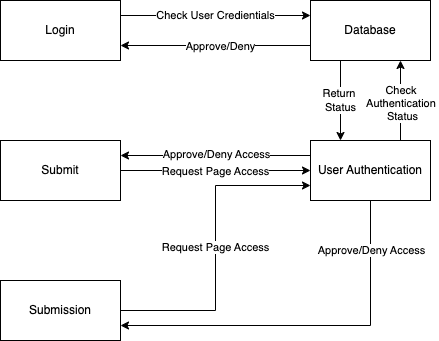
\includegraphics[width=0.75\textwidth]{Authentication.png}
\end{figure}

\newpage

\section{Appendix} \label{Appendix}

Add figma screenshots


\wss{Extra information if required}


\newpage{}

\section*{Appendix --- Reflection}

\begin{enumerate}
  \item What went well while writing this deliverable? 
  \item What pain points did you experience during this deliverable, and how
    did you resolve them?
  \item Which of your design decisions stemmed from speaking to your client(s)
  or a proxy (e.g. your peers, stakeholders, potential users)? For those that
  were not, why, and where did they come from?
  \item While creating the design doc, what parts of your other documents (e.g.
  requirements, hazard analysis, etc), it any, needed to be changed, and why?
  \item What are the limitations of your solution?  Put another way, given
  unlimited resources, what could you do to make the project better? (LO\_ProbSolutions)
  \item Give a brief overview of other design solutions you considered.  What
  are the benefits and tradeoffs of those other designs compared with the chosen
  design?  From all the potential options, why did you select the documented design?
  (LO\_Explores)
\end{enumerate}

\subsection*{Nathan Uy}

\begin{enumerate}
    \item I liked that our modules were very well-defined, making the writing of MIS easy.
    \item An issue I encountered was deciding which modules were necessary. It is very easy just to add as many modules as I want. To address this, every time I added a module, I ask myself does this module separate a distinct concern or responsibility? As a result, it limited the number of our modules to just the necessary ones.
\end{enumerate}

\subsection*{Declan Young}

\begin{enumerate}
    \item While writing this deliverable, creating the MIS for our application went well. This is because once we had broken the application into different modules with the MG, it was relatively straight-forward to create specification for these different modules, in order to satisfy the requirements of our application. 
    \item One of the pain points we encountered while writing this deliverable was determining how to break the application into different modules in the MG. This was a pain point because it was quite difficult to find a balance between breaking it into too many simple modules, versus not breaking it into enough modules, therefore leading to modules that were too general and complex. Another pain point was creating the timeline for all of the modules that needed to be implemented. This was difficult because it was hard to determine the complexity of the different modules in order to properly estimate the necessary time to complete it, as well as to fairly distribute the implementation of all the modules between team members fairly.
\end{enumerate}

\subsection*{Ben Dubois}

\begin{enumerate}
    \item While writing this deliverable, creating the MIS for each module went well as we already had each module clearly defined within the MG. This ensured that creating the MIS for each module was just adding a few extra details to each module and refining our definitions. 
    
    \item One of the pain points was creating the Use Hierarchy between modules. For this we had to determine which modules needed to be stand alone and which modules could use the existing features of another module. Therefore, for each new module we needed to look through all existing modules to see if there could be any use relation and this was time consuming. To resolve this, we started by defining all of the modules that we knew for sure could use an existing module and then created stand alone modules after this. This made the process much faster. 
\end{enumerate}

\subsection*{Aidan Mariglia}

\begin{enumerate}
    \item During this deliverable, the module decomposition went well. We were able to create clear lines of where the modules exist, defining the system structure and simplifying the process of implementation.
    
    \item Producing the access routine semantics for each module ahead of time was more of a pain point. Trying to foresee possible needs of modules which depend on other modules was difficult, and left me with the feeling there will be modifications needed when the implementation stage begins. 
\end{enumerate}

\subsection*{Team} 

\begin{enumerate}
\setcounter{enumi}{2}
    \item One of the major design decisions that originated from Dr. Kollmeyer was the design decisions regarding the user interface. Dr. Kollmeyer had a fairly specific vision for what the UI should look like, so after some discussions and elicitation of details, we were able to create the design consisting of both the different modules for the UI, as well as the visual design for the UI (which is seen in the Figma design). \\

    For the decisions that we did not consult our client, we instead brainstormed as a group for all major design decisions. We then ensured that all design decisions we made as a group followed the requirements for our application as well as it following the different properties/characteristics of design that we were trying to achieve.
    \item While creating our design document, we realized that the SRS document needed to be updated because we realized that some of our requirements were not necessary so those requirements were removed. Also, we noticed that some of our requirements were ambiguous and needed some clarification.
    \item One limitation of our solution is being able to display all the Matlab graphs for each submission due to limitations in our storage. In addition, with unlimited resources, we should be able to run more submissions concurrently, saving users time. 
    \item Another design we considered was only having one behavior hiding module, in an effort to reduce complexity. However, we came to the conclusion that although this would make implementation more simple, it would make maintenance and readability significantly worse.\\

    We ended up with our current design by ensuring it maintained a balanced of many of the different properties of design we prioritized, such as: Maintenance, complexity, readability and scalability 
\end{enumerate}


\end{document}